

\subsubsection{Results using post-EPS dataset}

We report the upper limits obtained using the data with the run number $<170826$ ( referred to 
as the EPS data) in the 0 and 1 jet bins separating the 
same flavor ($ee/\mu\mu$) and opposite flavor ($e\mu$) final states.
The observed and expected upper limits corresponding to the EPS data are shown in 
Figure~\ref{fig:limits_eps_cut}-\ref{fig:limits_eps_shape} for cut-based and multivariate 
based analyeses respectively, with the results tabulated in 
Table~\ref{tab:limits_eps_cut}-\ref{tab:limits_eps_shape} respectively.

%%%%%%%%%%%%%%%%%%%%%%%%%%%%%%
\begin{figure}[!htbp]
\centering
\subfigure[]{
\centering
\label{subfig:0j_sf}
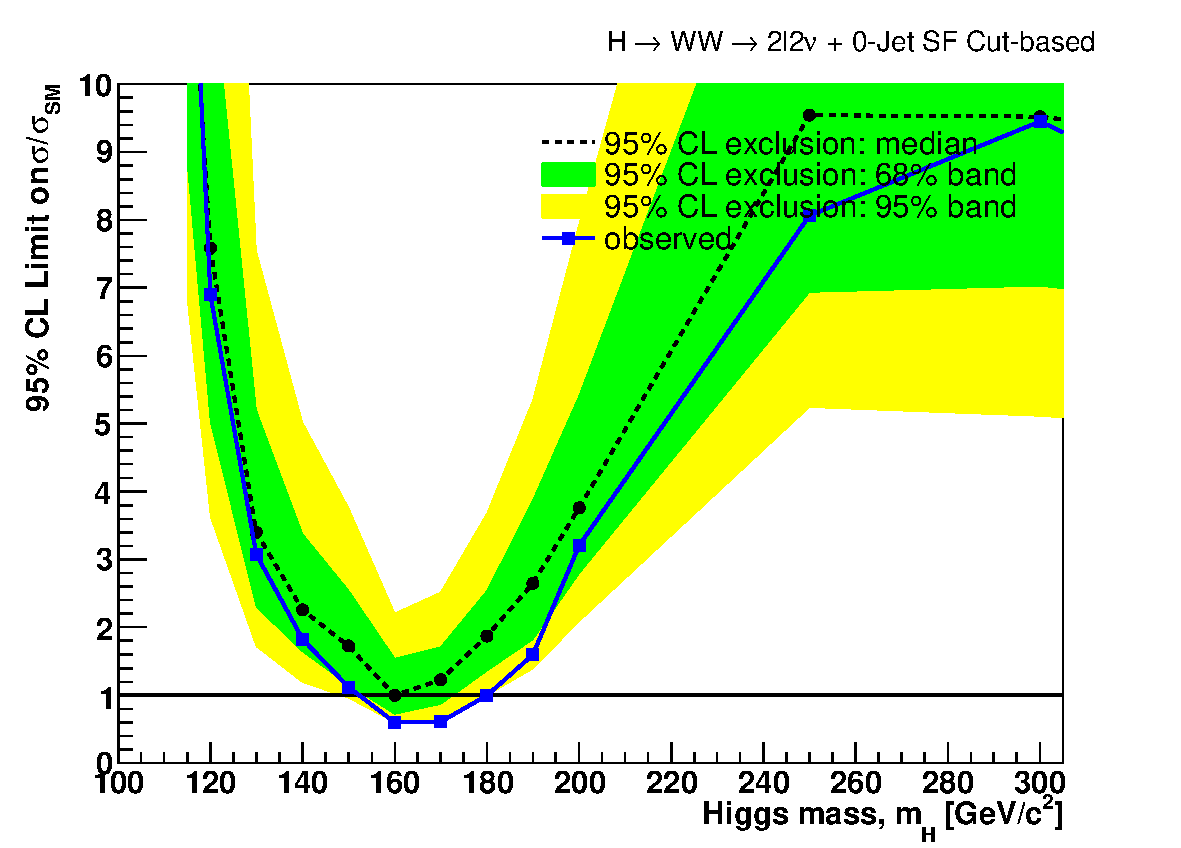
\includegraphics[width=0.48\textwidth]{lp_figures/limits_0j_sf_cut_ana_v6_1500pb_LP_POSTEPS.pdf}}
\subfigure[]{
\centering
\label{subfig:0j_of}
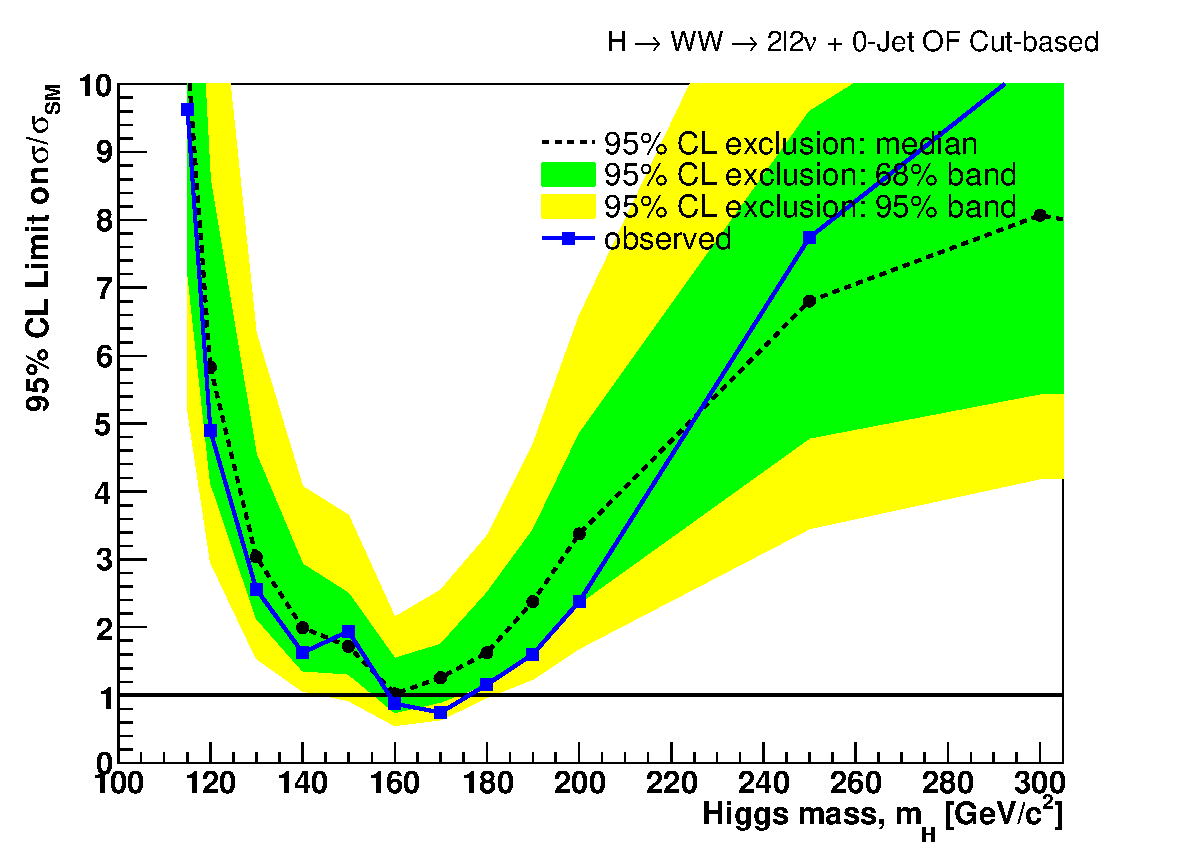
\includegraphics[width=0.48\textwidth]{lp_figures/limits_0j_of_cut_ana_v6_1500pb_LP_POSTEPS.pdf}}
\subfigure[]{
\centering
\label{subfig:1j_sf}
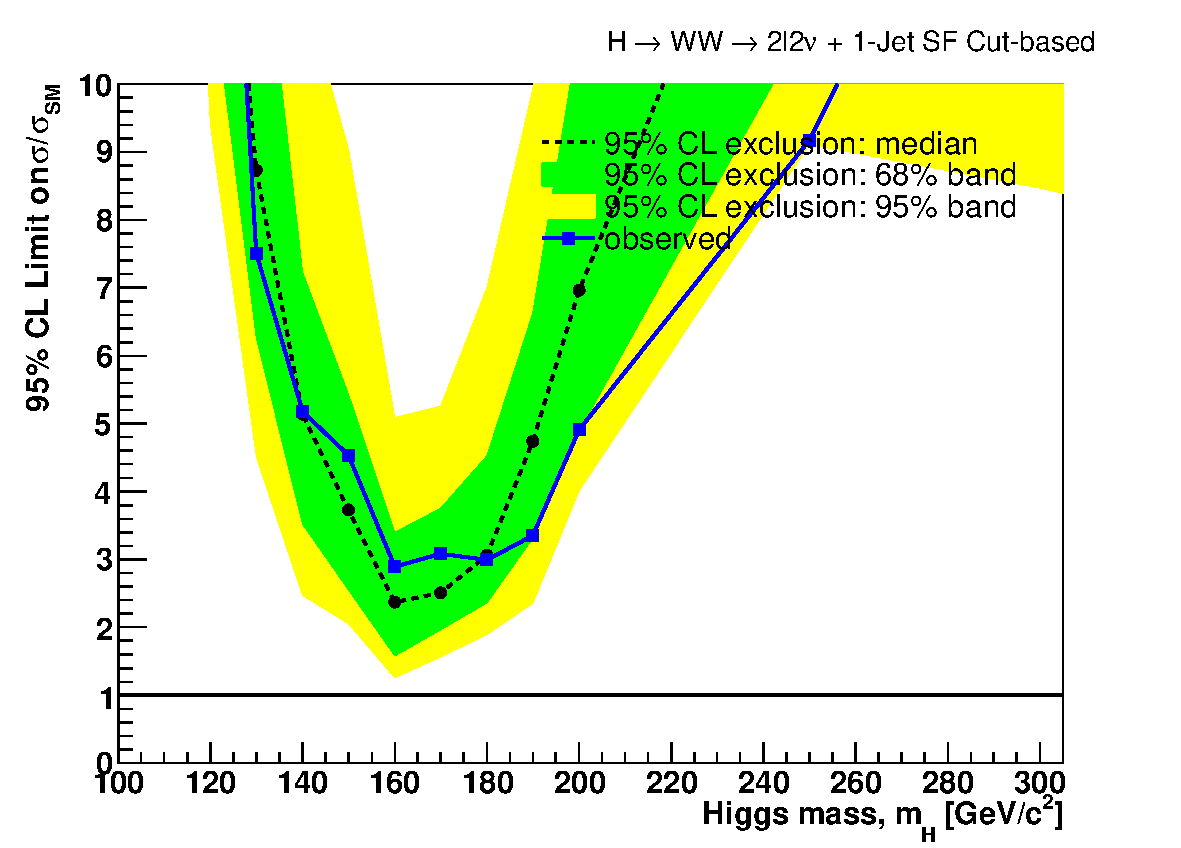
\includegraphics[width=0.48\textwidth]{lp_figures/limits_1j_sf_cut_ana_v6_1500pb_LP_POSTEPS.pdf}}
\subfigure[]{
\centering
\label{subfig:1j_of}
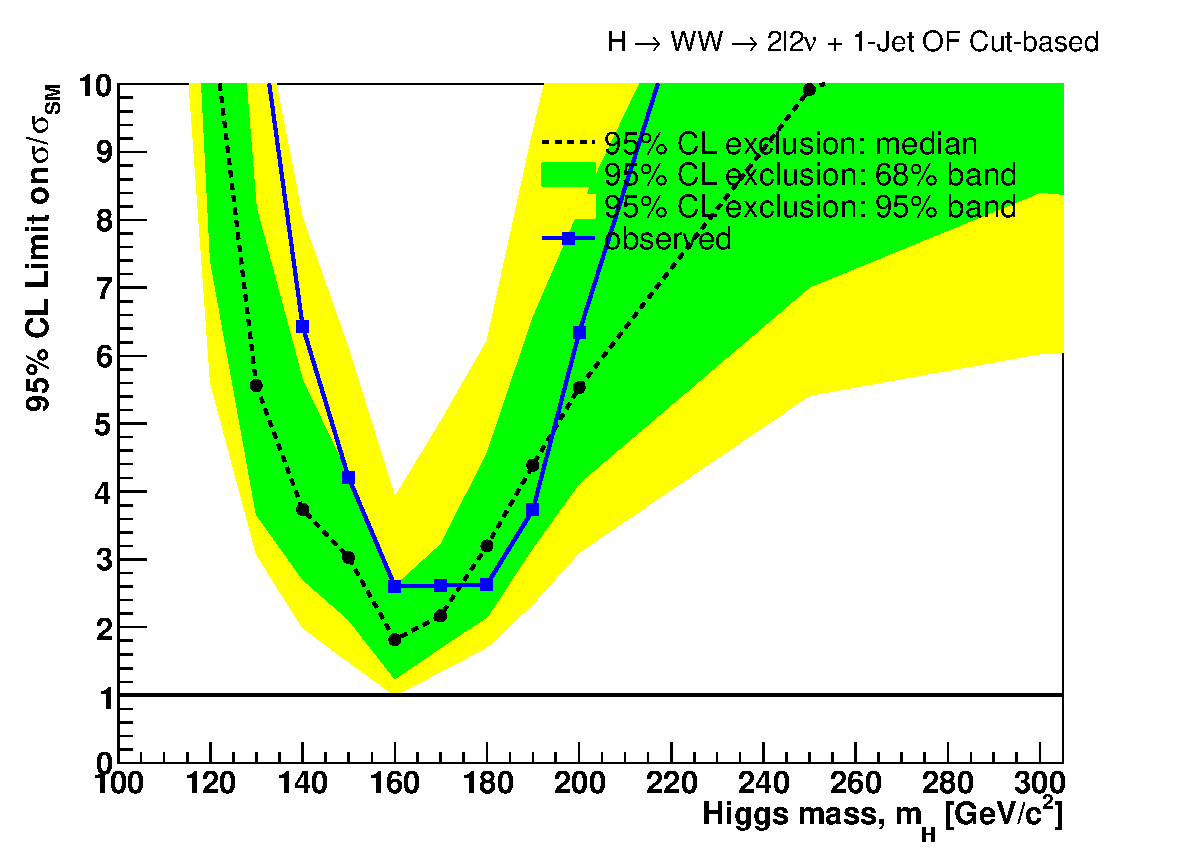
\includegraphics[width=0.48\textwidth]{lp_figures/limits_1j_of_cut_ana_v6_1500pb_LP_POSTEPS.pdf}}
\caption{Cut-based analysis upper limits at 95\% C.L. using the post-EPS data (run $>$ 170826) corresponding to 0.4~$\ifb$.
The limits are shown in 4 final states separately. \subref{subfig:0j_sf}: SF in 0 Jet bin; 
\subref{subfig:0j_of}: OF in 0 Jet bin; \subref{subfig:1j_sf}: SF in 1 Jet bin; 
\subref{subfig:1j_of}: OF in 1 Jet bin; 
}
\label{fig:limits_posteps_cut}
\end{figure}
%%%%%%%%%%%%%%%%%%%%%%%%%%%%%%

%%%%%%%%%%%%%%%%%%%%%%%%%%%%%%
\begin{figure}[!htbp]
\centering
\subfigure[]{
\centering
\label{subfig:0j_sf}
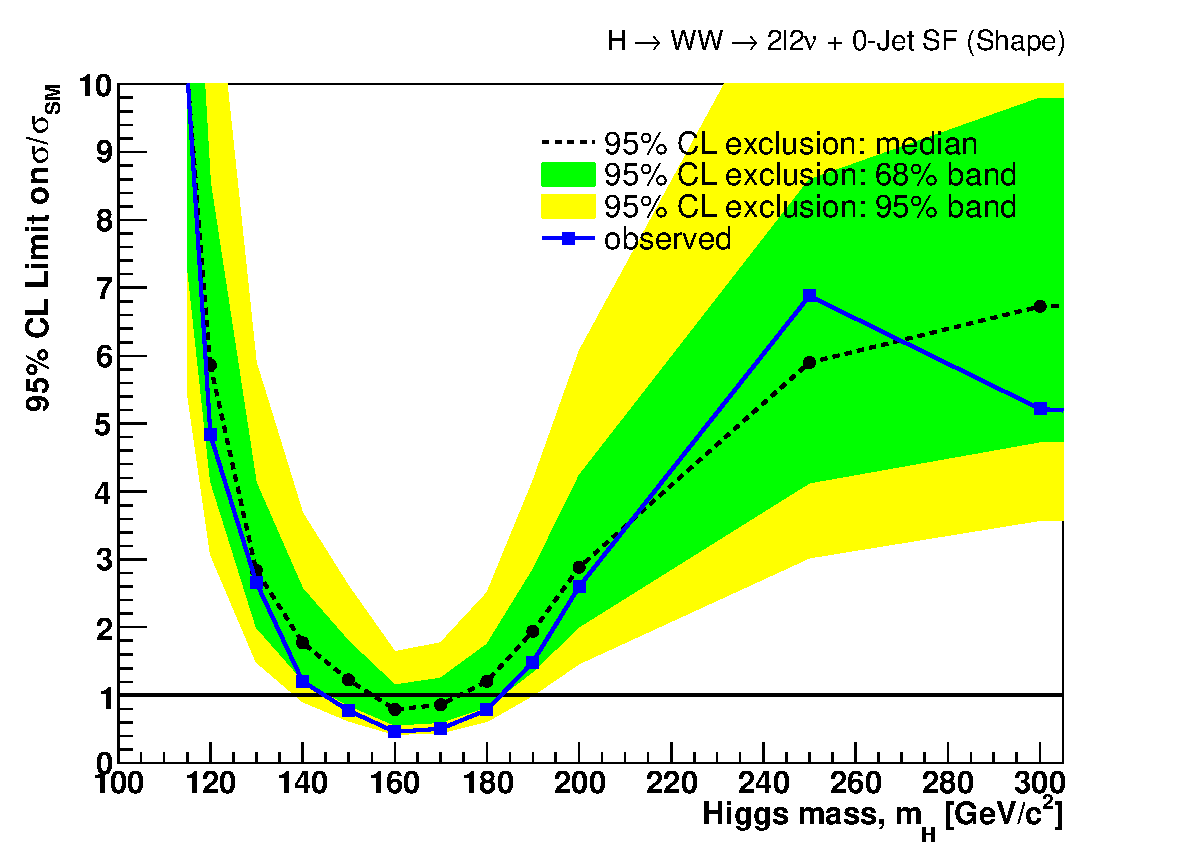
\includegraphics[width=0.48\textwidth]{lp_figures/limits_0j_sf_shape_ana_v6_1500pb_LP_POSTEPS.pdf}}
\subfigure[]{
\centering
\label{subfig:0j_of}
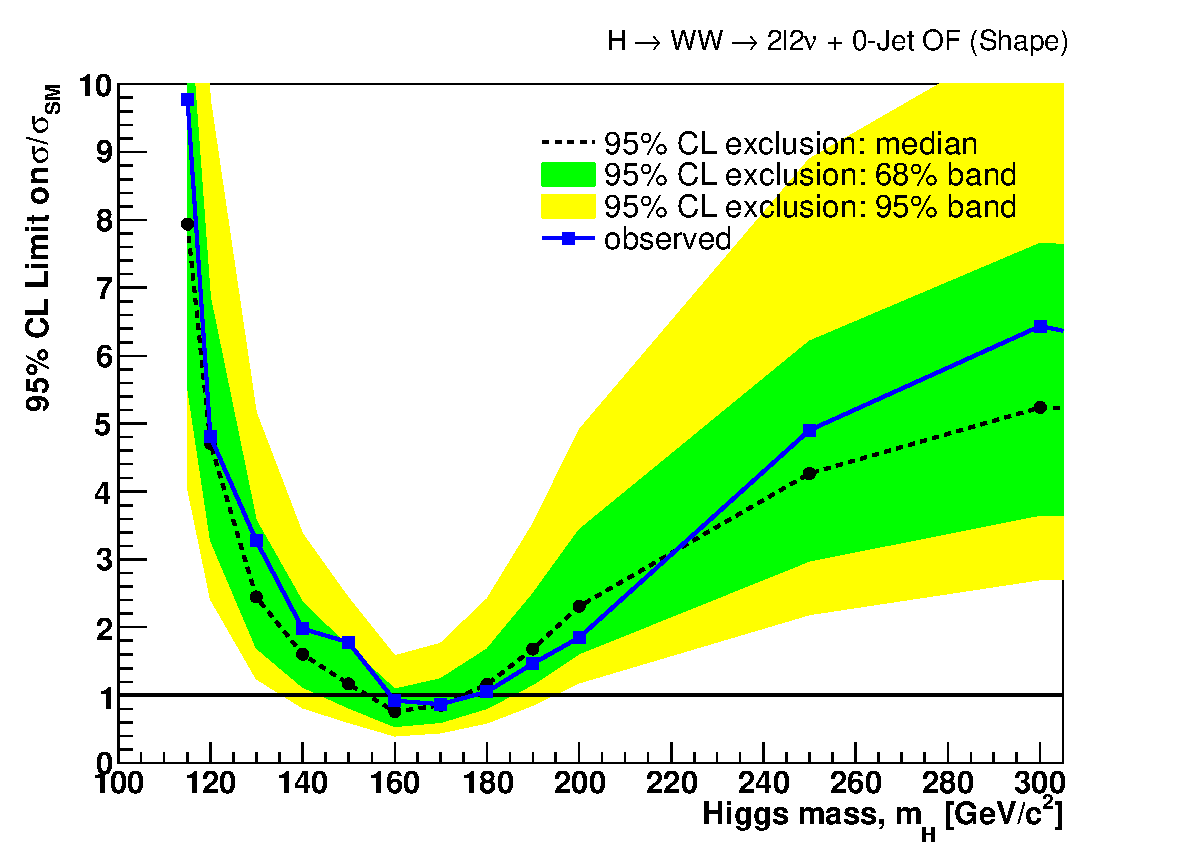
\includegraphics[width=0.48\textwidth]{lp_figures/limits_0j_of_shape_ana_v6_1500pb_LP_POSTEPS.pdf}}
\subfigure[]{
\centering
\label{subfig:1j_sf}
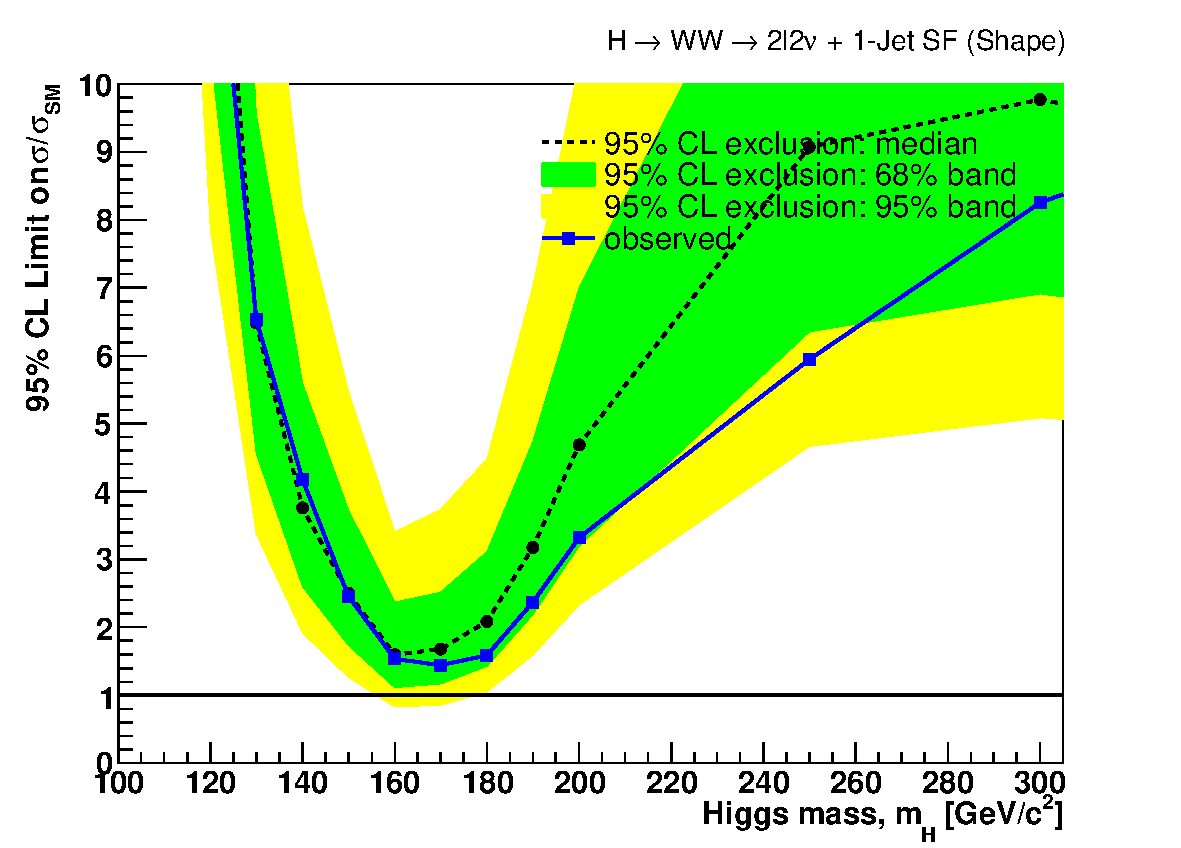
\includegraphics[width=0.48\textwidth]{lp_figures/limits_1j_sf_shape_ana_v6_1500pb_LP_POSTEPS.pdf}}
\subfigure[]{
\centering
\label{subfig:1j_of}
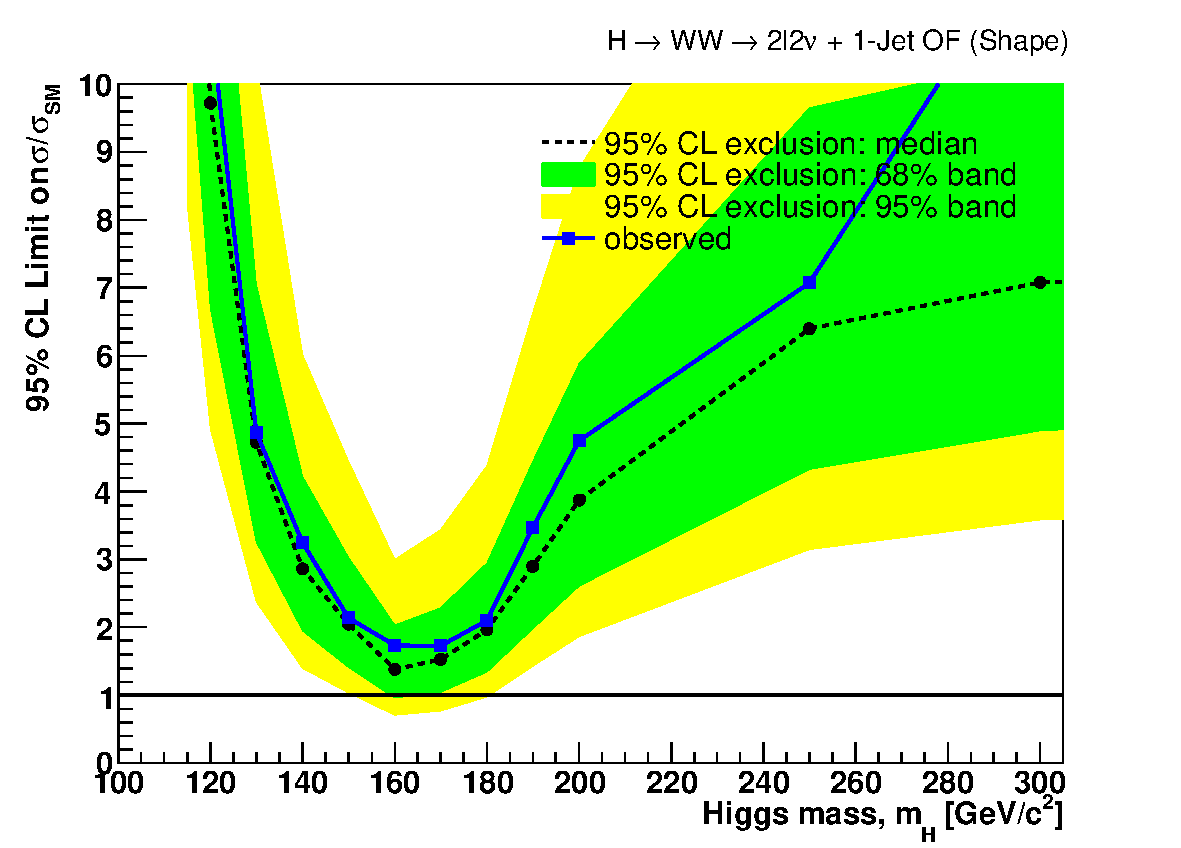
\includegraphics[width=0.48\textwidth]{lp_figures/limits_1j_of_shape_ana_v6_1500pb_LP_POSTEPS.pdf}}
\caption{Mutivariate based analysis upper limits at 95\% C.L. using the post-EPS data (run $>$ 170826) corresponding to 0.4~$\ifb$.
The limits are shown in 4 final states separately. \subref{subfig:0j_sf}: SF in 0 Jet bin; 
\subref{subfig:0j_of}: OF in 0 Jet bin; \subref{subfig:1j_sf}: SF in 1 Jet bin; 
\subref{subfig:1j_of}: OF in 1 Jet bin; 
}
\label{fig:limits_posteps_shape}
\end{figure}
%%%%%%%%%%%%%%%%%%%%%%%%%%%%%%

%%%%%%%%%%%%%%%%%%%%%%%%%%%%%%
\begin{table}
\begin{center}
\begin{tabular}{c c c c c}
\hline\hline
 $m_H$ (GeV) & Observed & Median Expected & 68\% C.L. Band & 95\% C.L. Band \\ \hline
\hline
\multicolumn{5}{c} {0-Jet Bin Same Flavor} \\
\hline
115 & 4.1 & 8.8 & [5.7, 15.4] & [4.0, 36.0] \\
120 & 4.1 & 5.0 & [3.2, 8.4] & [2.3, 17.6] \\
130 & 2.5 & 2.3 & [1.5, 3.4] & [1.0, 5.4] \\
140 & 1.6 & 1.5 & [1.0, 2.2] & [0.7, 3.3] \\
150 & 1.8 & 1.0 & [0.7, 1.5] & [0.5, 2.4] \\
160 & 1.0 & 0.6 & [0.4, 0.9] & [0.3, 1.6] \\
170 & 1.0 & 0.7 & [0.5, 1.0] & [0.3, 1.6] \\
180 & 0.6 & 1.0 & [0.7, 1.5] & [0.5, 2.2] \\
190 & 1.6 & 1.5 & [1.0, 2.1] & [0.7, 3.1] \\
200 & 2.1 & 2.2 & [1.6, 3.3] & [1.1, 4.6] \\
250 & 3.3 & 5.8 & [4.0, 8.5] & [3.0, 12.2] \\
300 & 4.3 & 5.5 & [3.9, 8.3] & [2.8, 11.9] \\
\hline
\multicolumn{5}{c} {0-Jet Bin Opposite Flavor} \\
\hline
115 & 7.6 & 6.6 & [4.5, 9.8] & [3.2, 14.4] \\
120 & 4.9 & 3.8 & [2.6, 5.7] & [1.9, 8.2] \\
130 & 2.8 & 1.9 & [1.3, 2.9] & [1.0, 4.2] \\
140 & 1.5 & 1.3 & [0.9, 1.8] & [0.6, 2.6] \\
150 & 0.9 & 1.0 & [0.7, 1.5] & [0.5, 2.2] \\
160 & 0.5 & 0.5 & [0.4, 0.8] & [0.3, 1.2] \\
170 & 0.7 & 0.7 & [0.5, 1.0] & [0.3, 1.4] \\
180 & 0.9 & 0.9 & [0.7, 1.4] & [0.5, 2.0] \\
190 & 1.4 & 1.3 & [0.9, 2.0] & [0.7, 2.8] \\
200 & 2.3 & 1.9 & [1.3, 2.8] & [1.0, 4.2] \\
250 & 3.1 & 3.9 & [2.8, 5.8] & [2.0, 8.2] \\
300 & 3.8 & 4.5 & [3.1, 6.6] & [2.3, 9.5] \\
\hline
\multicolumn{5}{c} {1-Jet Bin Same Flavor} \\
\hline
115 & 19.7 & 17.7 & [11.4, 26.5] & [8.6, 43.9] \\
120 & 12.4 & 9.4 & [6.4, 15.3] & [4.7, 27.8] \\
130 & 8.3 & 4.6 & [3.1, 7.2] & [2.1, 14.5] \\
140 & 5.7 & 2.7 & [1.7, 4.1] & [1.2, 7.0] \\
150 & 4.2 & 2.1 & [1.3, 3.2] & [1.0, 5.2] \\
160 & 2.3 & 1.1 & [0.8, 1.8] & [0.6, 2.7] \\
170 & 2.7 & 1.4 & [1.0, 2.1] & [0.7, 3.2] \\
180 & 2.9 & 1.8 & [1.3, 2.6] & [0.9, 3.8] \\
190 & 4.3 & 2.6 & [1.7, 4.0] & [1.3, 6.1] \\
200 & 6.5 & 4.0 & [2.7, 6.0] & [2.0, 9.4] \\
250 & 11.2 & 8.6 & [6.0, 13.2] & [4.4, 19.7] \\
300 & 12.1 & 8.7 & [6.0, 13.1] & [4.3, 19.5] \\
\hline
\multicolumn{5}{c} {1-Jet Bin Opposite Flavor} \\
\hline
115 & 19.4 & 10.2 & [6.9, 15.4] & [5.1, 22.9] \\
120 & 10.4 & 6.0 & [4.0, 8.9] & [3.0, 13.0] \\
130 & 4.1 & 3.2 & [2.1, 4.7] & [1.5, 7.2] \\
140 & 2.2 & 2.0 & [1.4, 3.0] & [1.0, 4.6] \\
150 & 1.6 & 1.6 & [1.1, 2.3] & [0.8, 3.5] \\
160 & 1.1 & 1.0 & [0.6, 1.4] & [0.5, 2.1] \\
170 & 1.2 & 1.2 & [0.8, 1.7] & [0.6, 2.7] \\
180 & 1.6 & 1.6 & [1.1, 2.5] & [0.9, 3.6] \\
190 & 2.1 & 2.6 & [1.8, 3.8] & [1.3, 5.6] \\
200 & 3.1 & 3.2 & [2.2, 4.8] & [1.6, 7.1] \\
250 & 6.2 & 6.1 & [4.2, 9.1] & [3.1, 13.6] \\
300 & 7.8 & 6.9 & [4.8, 10.4] & [3.5, 15.2] \\
\hline\hline
\end{tabular}
\end{center}
\caption{Cut-based upper limits at 95\% C.L. in 0 and 1 Jet final state, 
using the post-EPS data (run $>$ 170826) corresponding to  0.4~$\ifb$ 
shown in Figure~\ref{fig:limits_posteps_cut}.}
\label{tab:limits_posteps_cut}
\end{table}
%%%%%%%%%%%%%%%%%%%%%%%%%%%%%%
%%%%%%%%%%%%%%%%%%%%%%%%%%%%%%
\begin{table}
\begin{center}
\begin{tabular}{c c c c c}
\hline\hline
 $m_H$ (GeV) & Observed & Median Expected & 68\% C.L. Band & 95\% C.L. Band \\ \hline
\hline
\multicolumn{5}{c} {0-Jet Bin Same Flavor} \\
\hline
115 & 10.2 & 10.2 & [7.3, 14.7] & [5.4, 20.9] \\
120 & 4.8 & 5.9 & [4.2, 8.5] & [3.1, 12.4] \\
130 & 2.7 & 2.8 & [2.0, 4.1] & [1.5, 5.9] \\
140 & 1.2 & 1.8 & [1.2, 2.6] & [0.9, 3.7] \\
150 & 0.8 & 1.2 & [0.9, 1.8] & [0.6, 2.6] \\
160 & 0.5 & 0.8 & [0.6, 1.1] & [0.4, 1.6] \\
170 & 0.5 & 0.9 & [0.6, 1.2] & [0.4, 1.8] \\
180 & 0.8 & 1.2 & [0.8, 1.8] & [0.6, 2.5] \\
190 & 1.5 & 1.9 & [1.3, 2.8] & [1.0, 4.1] \\
200 & 2.6 & 2.9 & [2.0, 4.2] & [1.5, 6.1] \\
250 & 6.9 & 5.9 & [4.1, 8.6] & [3.0, 12.3] \\
300 & 5.2 & 6.7 & [4.7, 9.8] & [3.6, 14.0] \\
\hline
\multicolumn{5}{c} {0-Jet Bin Opposite Flavor} \\
\hline
115 & 9.8 & 7.9 & [5.5, 11.5] & [4.1, 16.5] \\
120 & 4.8 & 4.7 & [3.3, 6.9] & [2.4, 9.8] \\
130 & 3.3 & 2.4 & [1.7, 3.6] & [1.2, 5.2] \\
140 & 2.0 & 1.6 & [1.1, 2.4] & [0.8, 3.4] \\
150 & 1.8 & 1.2 & [0.8, 1.7] & [0.6, 2.4] \\
160 & 0.9 & 0.8 & [0.5, 1.1] & [0.4, 1.6] \\
170 & 0.9 & 0.9 & [0.6, 1.2] & [0.4, 1.8] \\
180 & 1.0 & 1.2 & [0.8, 1.7] & [0.6, 2.4] \\
190 & 1.5 & 1.7 & [1.2, 2.5] & [0.8, 3.5] \\
200 & 1.9 & 2.3 & [1.6, 3.4] & [1.2, 4.9] \\
250 & 4.9 & 4.3 & [3.0, 6.2] & [2.2, 8.9] \\
300 & 6.4 & 5.2 & [3.7, 7.7] & [2.7, 10.9] \\
\hline
\multicolumn{5}{c} {1-Jet Bin Same Flavor} \\
\hline
115 & 26.5 & 26.2 & [18.5, 38.7] & [14.1, 55.0] \\
120 & 13.4 & 15.0 & [10.5, 22.0] & [7.9, 32.3] \\
130 & 6.5 & 6.5 & [4.6, 9.6] & [3.4, 13.9] \\
140 & 4.2 & 3.8 & [2.6, 5.6] & [1.9, 8.2] \\
150 & 2.5 & 2.5 & [1.7, 3.7] & [1.3, 5.5] \\
160 & 1.5 & 1.6 & [1.1, 2.4] & [0.8, 3.4] \\
170 & 1.4 & 1.7 & [1.2, 2.5] & [0.9, 3.7] \\
180 & 1.6 & 2.1 & [1.4, 3.1] & [1.0, 4.5] \\
190 & 2.4 & 3.2 & [2.2, 4.7] & [1.6, 7.0] \\
200 & 3.3 & 4.7 & [3.2, 7.0] & [2.3, 10.3] \\
250 & 5.9 & 9.1 & [6.3, 13.6] & [4.7, 19.9] \\
300 & 8.3 & 9.8 & [6.9, 14.4] & [5.1, 20.9] \\
\hline
\multicolumn{5}{c} {1-Jet Bin Opposite Flavor} \\
\hline
115 & 20.2 & 15.9 & [11.1, 23.5] & [8.2, 33.6] \\
120 & 11.0 & 9.7 & [6.7, 14.3] & [4.9, 20.9] \\
130 & 4.9 & 4.7 & [3.3, 7.1] & [2.4, 10.3] \\
140 & 3.2 & 2.9 & [2.0, 4.2] & [1.4, 6.0] \\
150 & 2.1 & 2.0 & [1.4, 3.0] & [1.0, 4.4] \\
160 & 1.7 & 1.4 & [1.0, 2.0] & [0.7, 3.0] \\
170 & 1.7 & 1.5 & [1.0, 2.3] & [0.8, 3.4] \\
180 & 2.1 & 2.0 & [1.3, 2.9] & [1.0, 4.4] \\
190 & 3.5 & 2.9 & [2.0, 4.4] & [1.4, 6.6] \\
200 & 4.7 & 3.9 & [2.6, 5.9] & [1.9, 8.8] \\
250 & 7.1 & 6.4 & [4.3, 9.6] & [3.1, 14.1] \\
300 & 12.3 & 7.1 & [4.9, 10.4] & [3.6, 15.4] \\
\hline\hline
\end{tabular}
\end{center}
\caption{Multivariate based upper limits at 95\% C.L. in 0 and 1 Jet final state, 
using the post-EPS data (run $>$ 170826) corresponding to  0.4~$\ifb$ 
shown in Figure~\ref{fig:limits_posteps_shape}.}
\label{tab:limits_posteps_shape}
\end{table}
%%%%%%%%%%%%%%%%%%%%%%%%%%%%%%
\pagebreak

\subsubsection{Results using EPS dataset}
We report the upper limits obtained using the data with the run number 
$<170826$ ( referred to as the EPS data) in the 0 and 1 jet bins separating the 
same flavor ($ee/\mu\mu$) and opposite flavor ($e\mu$) final states.
The observed and expected upper limits corresponding to the EPS data are shown in 
Figure~\ref{fig:limits_eps_cut}-\ref{fig:limits_eps_shape} for cut-based and multivariate 
based analyeses respectively, with the results tabulated in 
Table~\ref{tab:limits_eps_cut}-\ref{tab:limits_eps_shape} respectively.


%%%%%%%%%%%%%%%%%%%%%%%%%%%%%%
\begin{figure}[!htbp]
\centering
\subfigure[]{
\centering
\label{subfig:0j_sf}
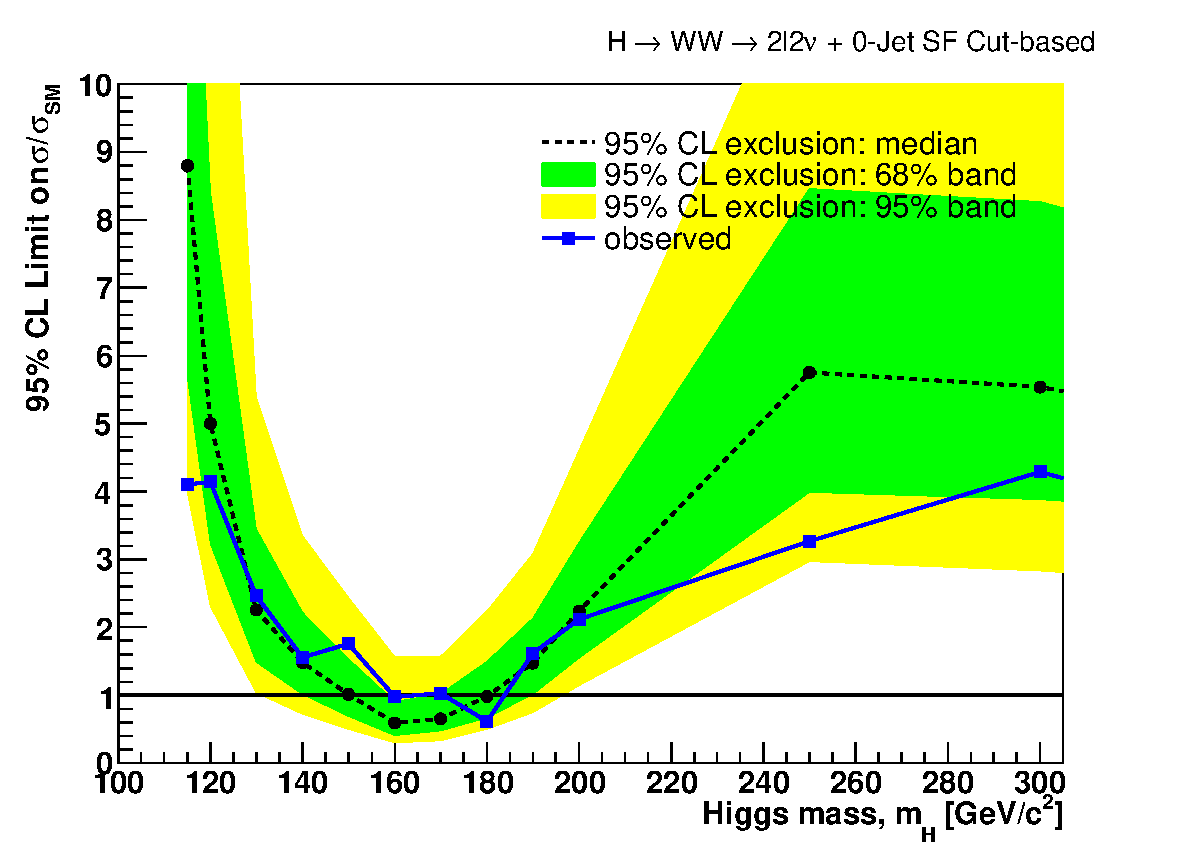
\includegraphics[width=0.48\textwidth]{lp_figures/limits_0j_sf_cut_ana_v6_1500pb_LP_EPS.pdf}}
\subfigure[]{
\centering
\label{subfig:0j_of}
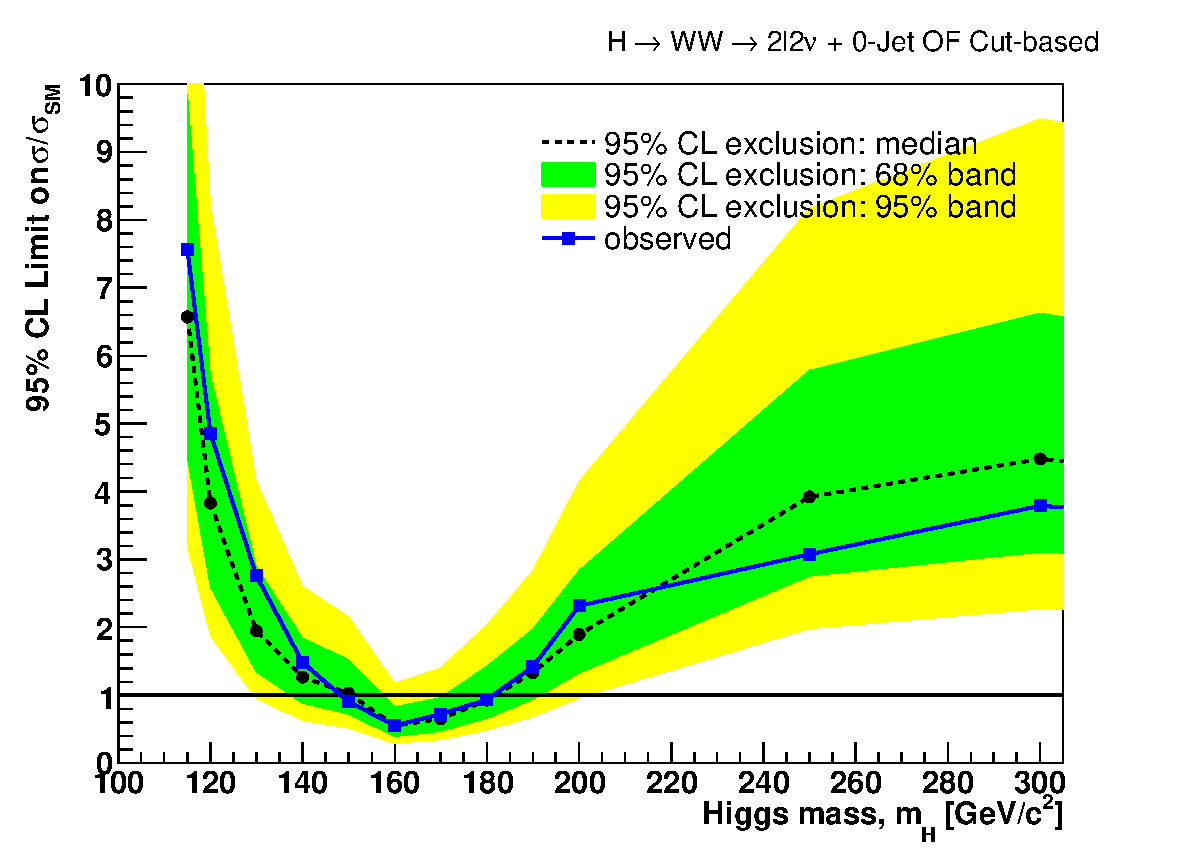
\includegraphics[width=0.48\textwidth]{lp_figures/limits_0j_of_cut_ana_v6_1500pb_LP_EPS.pdf}}
\subfigure[]{
\centering
\label{subfig:1j_sf}
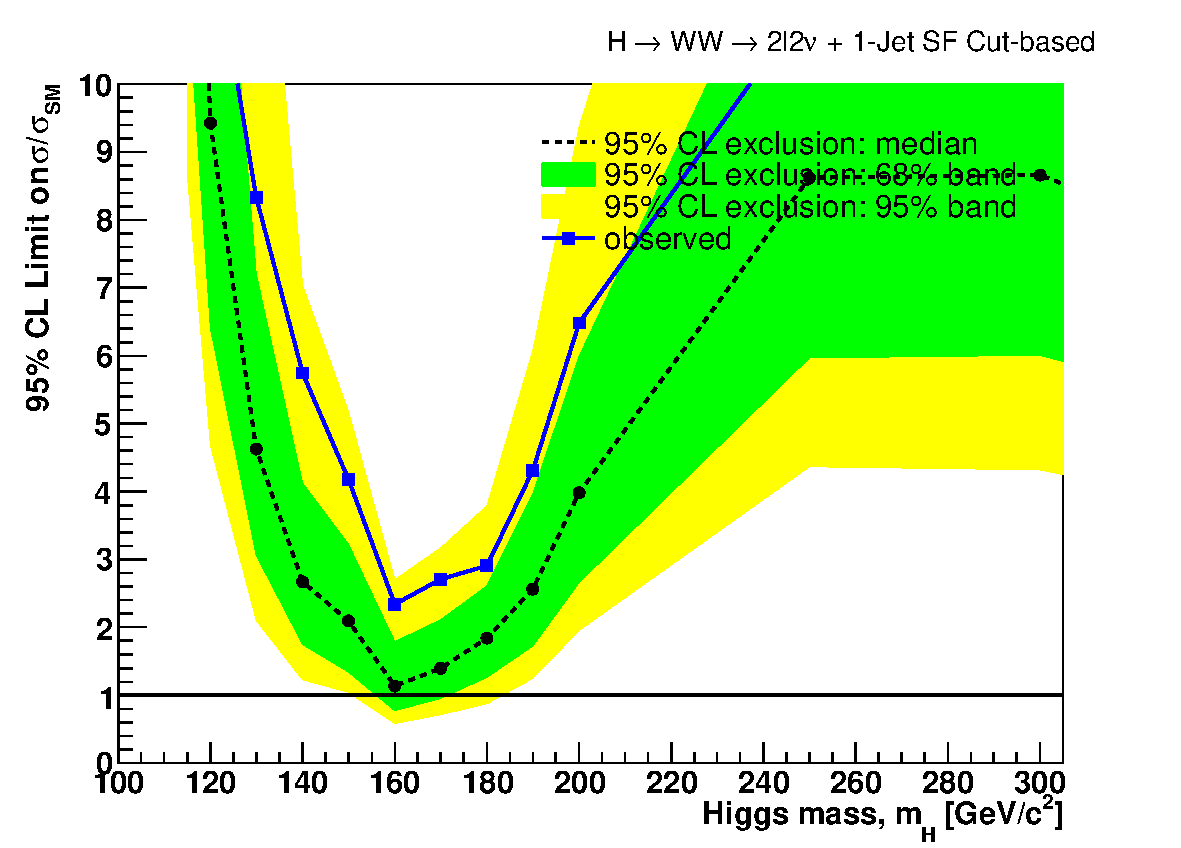
\includegraphics[width=0.48\textwidth]{lp_figures/limits_1j_sf_cut_ana_v6_1500pb_LP_EPS.pdf}}
\subfigure[]{
\centering
\label{subfig:1j_of}
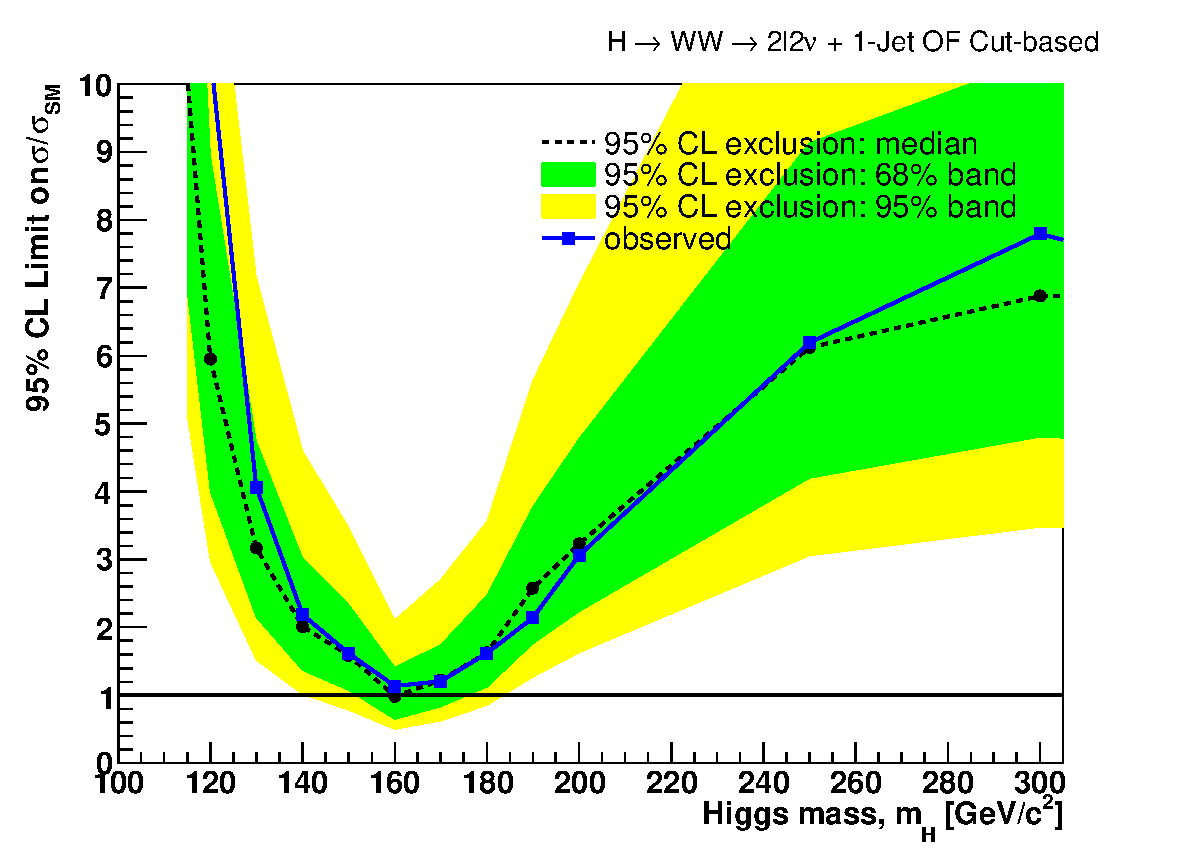
\includegraphics[width=0.48\textwidth]{lp_figures/limits_1j_of_cut_ana_v6_1500pb_LP_EPS.pdf}}
\caption{Cut-based analysis upper limits at 95\% C.L. using the EPS data (run $<=$ 170826) corresponding to 1.1~$\ifb$.
The limits are shown in 4 final states separately. \subref{subfig:0j_sf}: SF in 0 Jet bin; 
\subref{subfig:0j_of}: OF in 0 Jet bin; \subref{subfig:1j_sf}: SF in 1 Jet bin; 
\subref{subfig:1j_of}: OF in 1 Jet bin; 
}
\label{fig:limits_eps_cut}
\end{figure}
%%%%%%%%%%%%%%%%%%%%%%%%%%%%%%

%%%%%%%%%%%%%%%%%%%%%%%%%%%%%%
\begin{figure}[!htbp]
\centering
\subfigure[]{
\centering
\label{subfig:0j_sf}
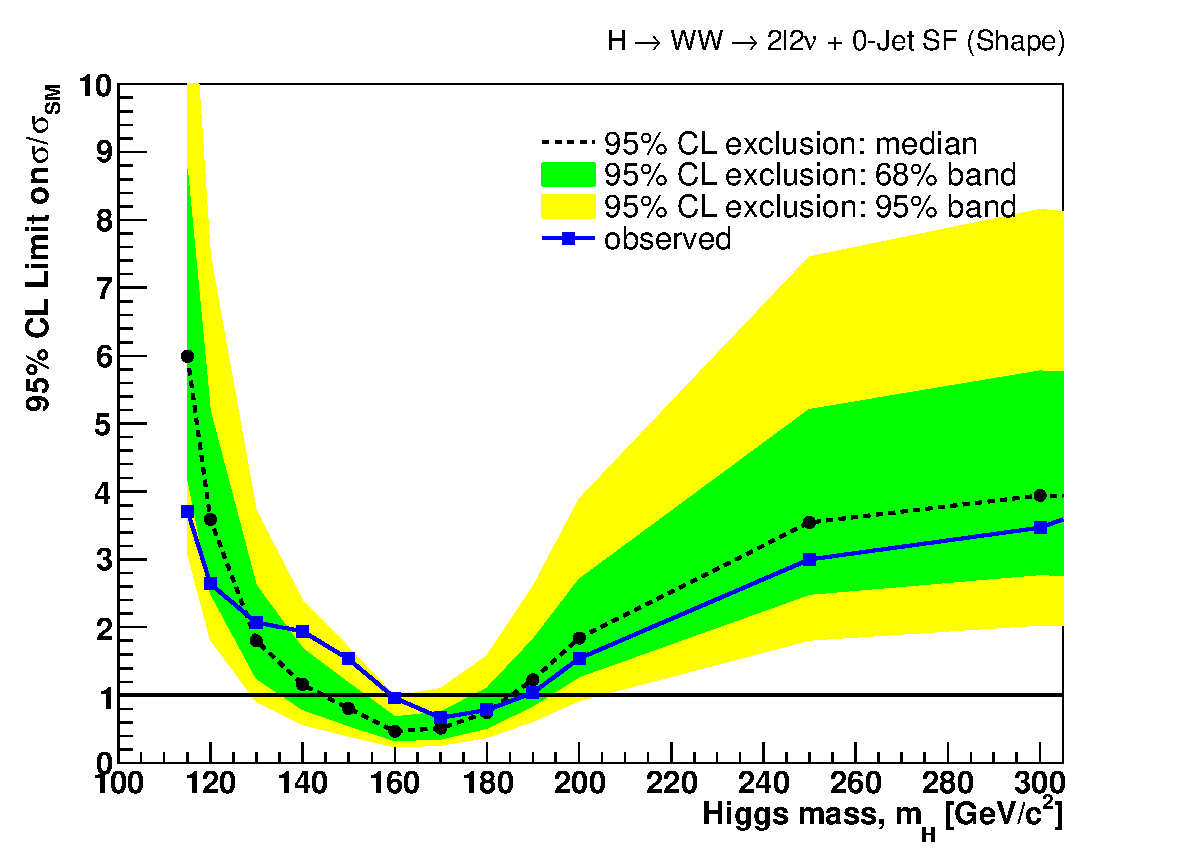
\includegraphics[width=0.48\textwidth]{lp_figures/limits_0j_sf_shape_ana_v6_1500pb_LP_EPS.pdf}}
\subfigure[]{
\centering
\label{subfig:0j_of}
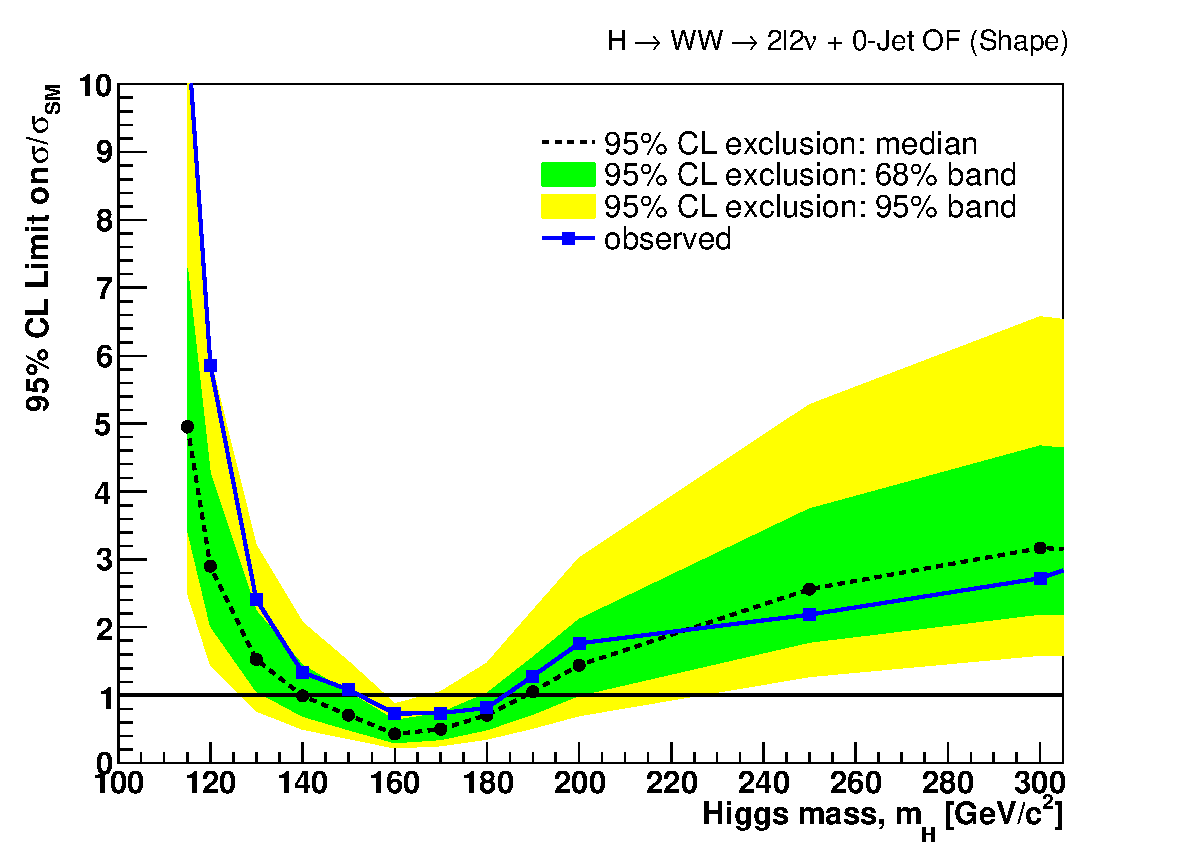
\includegraphics[width=0.48\textwidth]{lp_figures/limits_0j_of_shape_ana_v6_1500pb_LP_EPS.pdf}}
\subfigure[]{
\centering
\label{subfig:1j_sf}
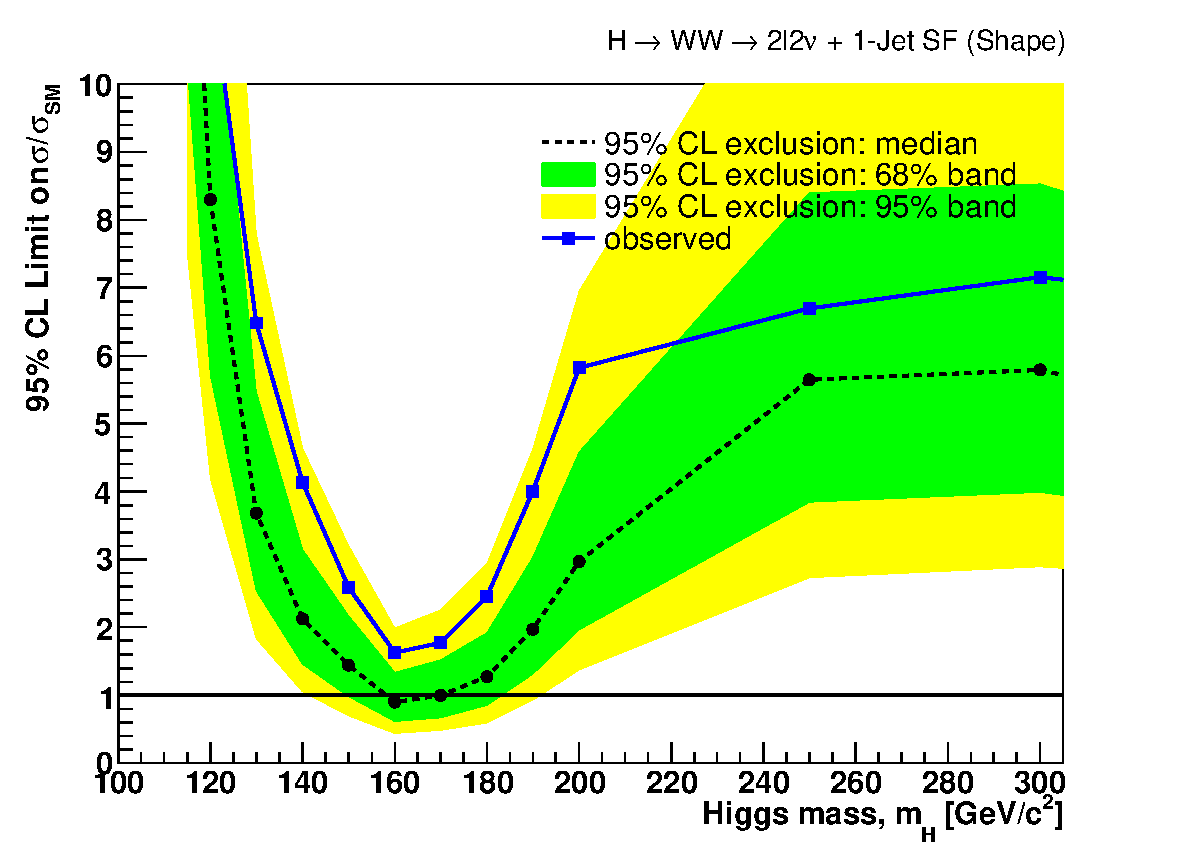
\includegraphics[width=0.48\textwidth]{lp_figures/limits_1j_sf_shape_ana_v6_1500pb_LP_EPS.pdf}}
\subfigure[]{
\centering
\label{subfig:1j_of}
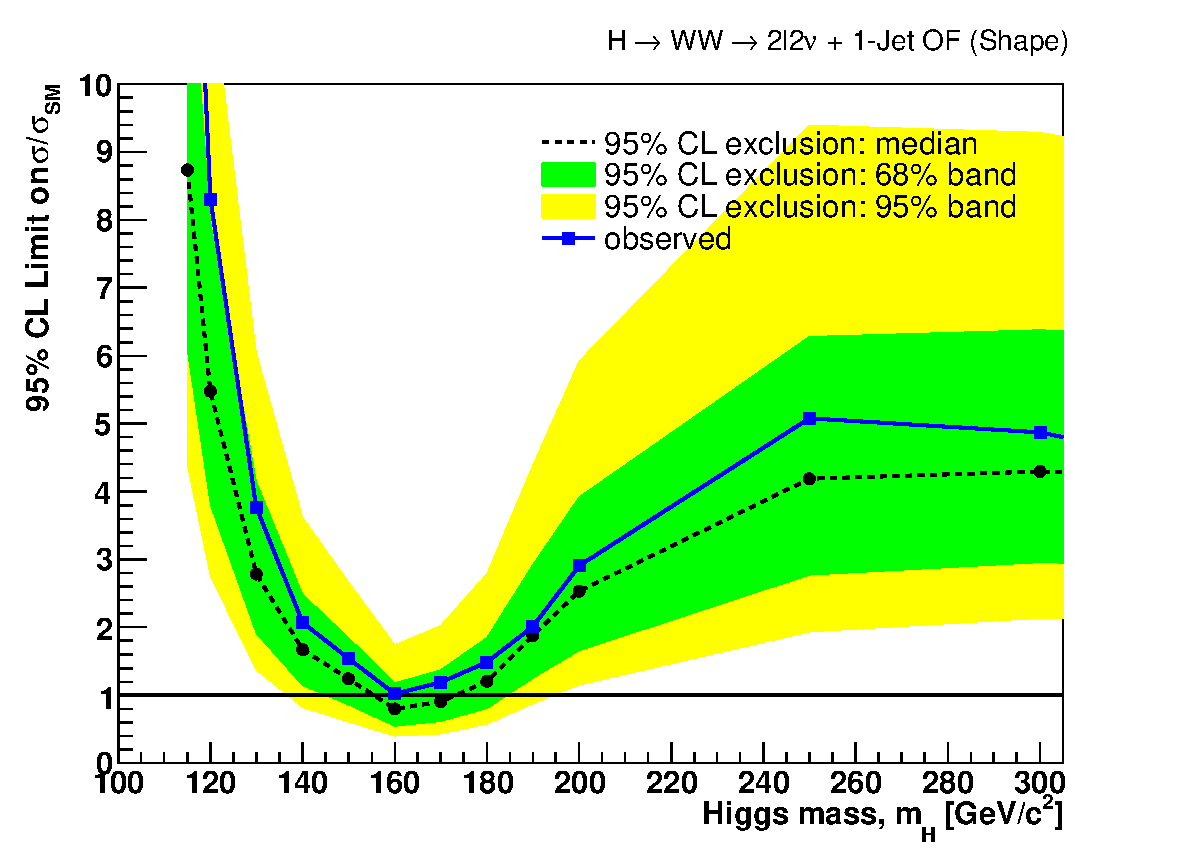
\includegraphics[width=0.48\textwidth]{lp_figures/limits_1j_of_shape_ana_v6_1500pb_LP_EPS.pdf}}
\caption{Multivariate based analysis upper limits at 95\% C.L. using the EPS data (run $<=$ 170826) corresponding to 1.1~$\ifb$.
The limits are shown in 4 final states separately. \subref{subfig:0j_sf}: SF in 0 Jet bin; 
\subref{subfig:0j_of}: OF in 0 Jet bin; \subref{subfig:1j_sf}: SF in 1 Jet bin; 
\subref{subfig:1j_of}: OF in 1 Jet bin; 
}
\label{fig:limits_eps_shape}
\end{figure}
%%%%%%%%%%%%%%%%%%%%%%%%%%%%%%

%%%%%%%%%%%%%%%%%%%%%%%%%%%%%%
\begin{table}
\begin{center}
\begin{tabular}{c c c c c}
\hline\hline
 $m_H$ (GeV) & Observed & Median Expected & 68\% C.L. Band & 95\% C.L. Band \\ \hline
\hline
\multicolumn{5}{c} {0-Jet Bin Same Flavor} \\
\hline
115 & 4.1 & 8.8 & [5.7, 15.4] & [4.0, 36.0] \\
120 & 4.1 & 5.0 & [3.2, 8.4] & [2.3, 17.6] \\
130 & 2.5 & 2.3 & [1.5, 3.4] & [1.0, 5.4] \\
140 & 1.6 & 1.5 & [1.0, 2.2] & [0.7, 3.3] \\
150 & 1.8 & 1.0 & [0.7, 1.5] & [0.5, 2.4] \\
160 & 1.0 & 0.6 & [0.4, 0.9] & [0.3, 1.6] \\
170 & 1.0 & 0.7 & [0.5, 1.0] & [0.3, 1.6] \\
180 & 0.6 & 1.0 & [0.7, 1.5] & [0.5, 2.2] \\
190 & 1.6 & 1.5 & [1.0, 2.1] & [0.7, 3.1] \\
200 & 2.1 & 2.2 & [1.6, 3.3] & [1.1, 4.6] \\
250 & 3.3 & 5.8 & [4.0, 8.5] & [3.0, 12.2] \\
300 & 4.3 & 5.5 & [3.9, 8.3] & [2.8, 11.9] \\
\hline
\multicolumn{5}{c} {0-Jet Bin Opposite Flavor} \\
\hline
115 & 7.6 & 6.6 & [4.5, 9.8] & [3.2, 14.4] \\
120 & 4.9 & 3.8 & [2.6, 5.7] & [1.9, 8.2] \\
130 & 2.8 & 1.9 & [1.3, 2.9] & [1.0, 4.2] \\
140 & 1.5 & 1.3 & [0.9, 1.8] & [0.6, 2.6] \\
150 & 0.9 & 1.0 & [0.7, 1.5] & [0.5, 2.2] \\
160 & 0.5 & 0.5 & [0.4, 0.8] & [0.3, 1.2] \\
170 & 0.7 & 0.7 & [0.5, 1.0] & [0.3, 1.4] \\
180 & 0.9 & 0.9 & [0.7, 1.4] & [0.5, 2.0] \\
190 & 1.4 & 1.3 & [0.9, 2.0] & [0.7, 2.8] \\
200 & 2.3 & 1.9 & [1.3, 2.8] & [1.0, 4.2] \\
250 & 3.1 & 3.9 & [2.8, 5.8] & [2.0, 8.2] \\
300 & 3.8 & 4.5 & [3.1, 6.6] & [2.3, 9.5] \\
\hline
\multicolumn{5}{c} {1-Jet Bin Same Flavor} \\
\hline
115 & 19.7 & 17.7 & [11.4, 26.5] & [8.6, 43.9] \\
120 & 12.4 & 9.4 & [6.4, 15.3] & [4.7, 27.8] \\
130 & 8.3 & 4.6 & [3.1, 7.2] & [2.1, 14.5] \\
140 & 5.7 & 2.7 & [1.7, 4.1] & [1.2, 7.0] \\
150 & 4.2 & 2.1 & [1.3, 3.2] & [1.0, 5.2] \\
160 & 2.3 & 1.1 & [0.8, 1.8] & [0.6, 2.7] \\
170 & 2.7 & 1.4 & [1.0, 2.1] & [0.7, 3.2] \\
180 & 2.9 & 1.8 & [1.3, 2.6] & [0.9, 3.8] \\
190 & 4.3 & 2.6 & [1.7, 4.0] & [1.3, 6.1] \\
200 & 6.5 & 4.0 & [2.7, 6.0] & [2.0, 9.4] \\
250 & 11.2 & 8.6 & [6.0, 13.2] & [4.4, 19.7] \\
300 & 12.1 & 8.7 & [6.0, 13.1] & [4.3, 19.5] \\
\hline
\multicolumn{5}{c} {1-Jet Bin Opposite Flavor} \\
\hline
115 & 19.4 & 10.2 & [6.9, 15.4] & [5.1, 22.9] \\
120 & 10.4 & 6.0 & [4.0, 8.9] & [3.0, 13.0] \\
130 & 4.1 & 3.2 & [2.1, 4.7] & [1.5, 7.2] \\
140 & 2.2 & 2.0 & [1.4, 3.0] & [1.0, 4.6] \\
150 & 1.6 & 1.6 & [1.1, 2.3] & [0.8, 3.5] \\
160 & 1.1 & 1.0 & [0.6, 1.4] & [0.5, 2.1] \\
170 & 1.2 & 1.2 & [0.8, 1.7] & [0.6, 2.7] \\
180 & 1.6 & 1.6 & [1.1, 2.5] & [0.9, 3.6] \\
190 & 2.1 & 2.6 & [1.8, 3.8] & [1.3, 5.6] \\
200 & 3.1 & 3.2 & [2.2, 4.8] & [1.6, 7.1] \\
250 & 6.2 & 6.1 & [4.2, 9.1] & [3.1, 13.6] \\
300 & 7.8 & 6.9 & [4.8, 10.4] & [3.5, 15.2] \\
\hline\hline
\end{tabular}
\end{center}
\caption{Cut based upper limits at 95\% C.L. in 0 and 1 Jet final state, 
using the EPS data (run $<=$ 170826) corresponding to  1.1~$\ifb$ 
shown in Figure~\ref{fig:limits_eps_cut}.}
\label{tab:limits_eps_cut}
\end{table}
%%%%%%%%%%%%%%%%%%%%%%%%%%%%%%

%%%%%%%%%%%%%%%%%%%%%%%%%%%%%%
\begin{table}
\begin{center}
\begin{tabular}{c c c c c}
\hline\hline
 $m_H$ (GeV) & Observed & Median Expected & 68\% C.L. Band & 95\% C.L. Band \\ \hline
\hline
\multicolumn{5}{c} {0-Jet Bin Same Flavor} \\
\hline
115 & 3.7 & 6.0 & [4.2, 8.7] & [3.1, 12.6] \\
120 & 2.6 & 3.6 & [2.5, 5.2] & [1.8, 7.5] \\
130 & 2.1 & 1.8 & [1.2, 2.6] & [0.9, 3.7] \\
140 & 1.9 & 1.2 & [0.8, 1.7] & [0.6, 2.4] \\
150 & 1.5 & 0.8 & [0.6, 1.2] & [0.4, 1.7] \\
160 & 1.0 & 0.5 & [0.3, 0.7] & [0.2, 1.0] \\
170 & 0.7 & 0.5 & [0.4, 0.8] & [0.3, 1.1] \\
180 & 0.8 & 0.7 & [0.5, 1.1] & [0.4, 1.6] \\
190 & 1.0 & 1.2 & [0.8, 1.8] & [0.6, 2.6] \\
200 & 1.5 & 1.8 & [1.3, 2.7] & [0.9, 3.9] \\
250 & 3.0 & 3.5 & [2.5, 5.2] & [1.8, 7.5] \\
300 & 3.5 & 3.9 & [2.8, 5.8] & [2.0, 8.2] \\
\hline
\multicolumn{5}{c} {0-Jet Bin Opposite Flavor} \\
\hline
115 & 10.9 & 5.0 & [3.4, 7.3] & [2.5, 10.5] \\
120 & 5.9 & 2.9 & [2.0, 4.3] & [1.4, 5.9] \\
130 & 2.4 & 1.5 & [1.1, 2.2] & [0.8, 3.2] \\
140 & 1.3 & 1.0 & [0.7, 1.4] & [0.5, 2.1] \\
150 & 1.1 & 0.7 & [0.5, 1.0] & [0.4, 1.5] \\
160 & 0.7 & 0.4 & [0.3, 0.6] & [0.2, 0.9] \\
170 & 0.7 & 0.5 & [0.3, 0.7] & [0.3, 1.1] \\
180 & 0.8 & 0.7 & [0.5, 1.0] & [0.4, 1.5] \\
190 & 1.3 & 1.1 & [0.7, 1.6] & [0.5, 2.2] \\
200 & 1.8 & 1.4 & [1.0, 2.1] & [0.7, 3.0] \\
250 & 2.2 & 2.6 & [1.8, 3.7] & [1.3, 5.3] \\
300 & 2.7 & 3.2 & [2.2, 4.7] & [1.6, 6.6] \\
\hline
\multicolumn{5}{c} {1-Jet Bin Same Flavor} \\
\hline
115 & 24.4 & 14.8 & [10.3, 21.7] & [7.5, 30.8] \\
120 & 11.5 & 8.3 & [5.7, 12.2] & [4.2, 17.9] \\
130 & 6.5 & 3.7 & [2.5, 5.5] & [1.8, 7.8] \\
140 & 4.1 & 2.1 & [1.5, 3.1] & [1.1, 4.6] \\
150 & 2.6 & 1.4 & [1.0, 2.2] & [0.7, 3.2] \\
160 & 1.6 & 0.9 & [0.6, 1.3] & [0.4, 2.0] \\
170 & 1.8 & 1.0 & [0.7, 1.5] & [0.5, 2.3] \\
180 & 2.5 & 1.3 & [0.8, 1.9] & [0.6, 2.9] \\
190 & 4.0 & 2.0 & [1.3, 3.0] & [0.9, 4.6] \\
200 & 5.8 & 3.0 & [2.0, 4.6] & [1.4, 6.9] \\
250 & 6.7 & 5.6 & [3.8, 8.4] & [2.7, 12.5] \\
300 & 7.2 & 5.8 & [4.0, 8.5] & [2.9, 12.2] \\
\hline
\multicolumn{5}{c} {1-Jet Bin Opposite Flavor} \\
\hline
115 & 15.8 & 8.7 & [6.1, 12.8] & [4.4, 18.3] \\
120 & 8.3 & 5.5 & [3.8, 8.0] & [2.8, 11.6] \\
130 & 3.8 & 2.8 & [1.9, 4.2] & [1.4, 6.0] \\
140 & 2.1 & 1.7 & [1.1, 2.5] & [0.8, 3.6] \\
150 & 1.5 & 1.2 & [0.9, 1.9] & [0.6, 2.7] \\
160 & 1.0 & 0.8 & [0.5, 1.2] & [0.4, 1.7] \\
170 & 1.2 & 0.9 & [0.6, 1.4] & [0.4, 2.0] \\
180 & 1.5 & 1.2 & [0.8, 1.8] & [0.6, 2.8] \\
190 & 2.0 & 1.9 & [1.2, 2.9] & [0.9, 4.4] \\
200 & 2.9 & 2.5 & [1.7, 3.9] & [1.2, 5.9] \\
250 & 5.1 & 4.2 & [2.8, 6.3] & [1.9, 9.4] \\
300 & 4.9 & 4.3 & [3.0, 6.4] & [2.1, 9.3] \\
\hline\hline
\end{tabular}
\end{center}
\caption{Multivariate based upper limits at 95\% C.L. in 0 and 1 Jet final state, 
using the EPS data (run $<=$ 170826) corresponding to  1.1~$\ifb$ 
shown in Figure~\ref{fig:limits_eps_shape}.}
\label{tab:limits_eps_shape}
\end{table}
%%%%%%%%%%%%%%%%%%%%%%%%%%%%%%
\pagebreak